% Generated by scripts/paper_tex.py from paper.html; edit the HTML source (web/app/paper_src), not this file.
\documentclass[twocolumn]{aastex631}
\usepackage{xeCJK}
\setCJKmainfont{Noto Serif CJK TC}[BoldFont={Noto Serif CJK TC Bold}]
\setCJKsansfont{Noto Sans CJK TC}
\setCJKmonofont{Noto Sans Mono CJK TC}
\xeCJKsetup{CJKspace=true}
\usepackage{graphicx}
\usepackage{tabularx}
\renewcommand{\figurename}{圖}\renewcommand{\tablename}{表}\renewcommand{\abstractname}{摘要}\renewcommand{\refname}{參考文獻}\renewcommand{\appendixname}{附錄}
\shorttitle{SPHEREx 影像中的移動天體}
\shortauthors{SPHEREx Sky Change}
\begin{document}
\title{用只以模擬資料訓練的真假訊號網路與視差串連，在 SPHEREx 全天光譜影像中尋找移動天體}
\author{SPHEREx Sky Change 團隊}
\affiliation{NASA Space Apps Challenge 2026 · Planet X and SPHEREx}
\begin{abstract}
SPHEREx 每六個月以 102 個近紅外線波段拍攝全天，成為尋找移動天體的新工具：小行星、彗星，原則上也包括尚未發現的遙遠行星。但它的設計也讓變化偵測變得困難：每個偵測器裝有線性漸變濾鏡，影像中不同位置的波長不同；點擴散函數欠取樣（半高寬約 5$''$，像素 6.15$''$）；同一片天空的連續影像又是在不同波長拍的。我們建立的管線會：（i）把 0.5$^\circ$ 天區的每張曝光重新取樣到同一個天空網格；（ii）對每個像素，用同一個偵測器、該像素波長相差 3\% 以內、且相隔至少 3 小時的曝光建立參考影像；（iii）偵測 5$\sigma$ 的正殘差；（iv）用卷積神經網路為每個候選評分；（v）把偵測串成直線軌跡，或跨巡天輪次串成符合地球視差的軌跡。網路在訓練時從沒看過真實小行星，只學過以儀器自身 PSF 注入的移動天體和真實的假訊號。在 19 個從未用於訓練的天區裡，它把 556 次真實已知小行星的偵測和同一批天區的假訊號分開，AUROC 為 0.987（95\% CI 0.981--0.992），在誤報率 1.15\% 時保留其中 90.8\%。比對到的偵測和 JPL 對太空船的預測位置相差中位數 0.7$''$。注入天體在單張曝光的 50\% 完整度為 AB 17.3。沿圓軌道運動的注入遠距天體，靠視差加上擬合的軌道運動在有三輪巡天的天區找回了 47/48 顆（只有兩輪的天區依設計找不回）；先前一版在注入與擬合中都忽略了軌道運動，屬於循環驗證，我們如實報告。我們也報告兩個關鍵的失誤：一個把真實移動天體的訊噪比壓在 10 左右的雜訊模型，以及一個只會出現在真實移動天體、從不出現在模擬天體上的處理管線旗標。只靠 SPHEREx 的視差，盲搜尋量出兩顆真實矮行星的距離：鳥神星 52.71 AU（JPL 52.72，差 0.02\%）、妊神星 49.49 AU（JPL 49.82，差 0.66\%）。沿 Planet Nine 預測路徑與 2025 年 IRAS/AKARI 候選附近搜尋 32 片天空（7.89 平方度）：單張影像沒有任何遠距軌跡；移位疊加（50\% 完整度 AB 19.2）連出 63 條軌跡，但數量和打亂巡天時間後的巧合（55 與 60 條）相當。我們沒有發現新行星；注入測試與這個非偵測，呈現的是這個方法做得到與做不到的範圍。

\medskip\noindent\textbf{重點}
\begin{itemize}\setlength{\itemsep}{1pt}
\item 針對 SPHEREx 線性漸變濾鏡設計的差分影像管線，逐像素依波長配對參考影像，能在單張約 2 分鐘的曝光中偵測移動天體。
\item 只用注入天體訓練的 32 萬參數 CNN，在 19 個從未用於訓練的天區裡，把 556 次真實已知小行星的偵測和同一批天區的假訊號分開，AUROC 0.987；只看訊噪比只有 0.537。
\item 跨巡天輪次同時擬合距離與軌道運動，在有三輪巡天的天區找回 48 顆沿圓軌道運動的注入遠距天體（500--3000 AU）中的 47 顆（只有兩輪的天區一顆也找不回），距離誤差中位數 0.09\%。
\item 已知小行星的位置和 JPL Horizons 以 SPHEREx 太空船為觀測者算出的預測相差中位數 0.7$''$（0.11 個像素；6 個天體、78 次偵測）。
\end{itemize}
\noindent{\footnotesize 黑客松技術報告，未經同儕審查。網站與資料：\url{https://quilt-advocate-boys-recovered.trycloudflare.com}}
\end{abstract}
\keywords{小行星 --- 海王星外天體 --- 天文影像處理 --- 卷積神經網路 --- 視差}


\section{前言}
\label{sec:intro}
2026 年 Space Apps 的題目要求做一個公開的網頁工具，顯示 SPHEREx 拍到的天空，讓人容易看出天空隨時間的變化。小行星、彗星、鄰近恆星、棕矮星，甚至新的行星，都會因為在影像之間移動而露出行蹤。Backyard Worlds（Kuchner et al., 2017）證明了大眾能靠閃爍比對 WISE 影像找到移動天體。SPHEREx（Doré et al., 2014）的資料更豐富，但直接閃爍它的原始影像會誤導人：同一顆恆星在不同波長拍到的樣子本來就不同，即使它完全沒動。

因此我們在公開檢視器背後放了一條經過量測的偵測管線，讓大家看到的東西都先通過定量檢驗。我們檢驗三個假說（判準及設定的時點見附錄 A）：

\begin{itemize}
\item \textbf{H1.} 只用模擬移動天體訓練的網路，辨識真實已知小行星的 AUROC $\ge$ 0.95。
\item \textbf{H2.} 逐像素波長配對加上以參考影像亮度為準的誤差項，能讓每個偵測器在選定操作點的誤報率都維持在低水準。
\item \textbf{H3.} 巡天輪次之間的地球視差，能把注入遠距天體的距離量到 2\% 以內。
\end{itemize}

\section{資料}
\label{sec:data}
我們使用 NASA/IPAC IRSA 提供的 SPHEREx Quick Release 第 2 級光譜影像（\texttt{spherex\_qr2} 與 \texttt{spherex\_qr3}），涵蓋 2025 年 5 月至 2026 年 9 月：三輪全天巡天和第四輪的一部分。每張曝光約 3.5$^\circ$ $\times$ 3.5$^\circ$，來自六個偵測器之一（D1--D6，0.75--5.0 $\mu$m）。我們透過 IRSA 的影像裁切服務取得 cutout，使用 IMAGE（減去 ZODI）、VARIANCE、FLAGS、逐像素波長表（\texttt{WAVE-TAB} WCS）與 PSF 立方體（11 $\times$ 11 個偵測器區域、10 倍過取樣）。QR3 檔案改用 \texttt{EPSF} 表格而沒有 PSF 立方體；對 QR3 曝光做注入時，我們沿用同一偵測器在 QR2 的 PSF 立方體。

16 個 0.5$^\circ$ 天區沿黃道每 30$^\circ$ 經度取一個（$\beta$ = 0$^\circ$ 或 3$^\circ$），另有 4 個在 |$\beta$| = 12$^\circ$。另外 15 個天區以 13 $\le$ V $\le$ 17 的小行星為中心：我們在 6 個日期、SPHEREx 正在觀測的黃道經度上，用 JPL Small-Body Identification API 找出這些小行星；它們只用於評估。每個觀測時段（0.5 天內的曝光）的已知天體同樣來自這個 API（V $\le$ 21.5），位置在時段內線性外推。

\begin{table*}[t]
\centering
\footnotesize

\begin{tabular}{llllll}
\hline\hline
用途 & 天區 & 候選 & 注入 & 已知小行星 (V$\le$18.5) & 假訊號 \\
\hline
訓練 & 12 & 729,286 & 12,351 & 199 & 716,736 \\
驗證 & 2 & 68,573 & 2,227 & 27 & 66,319 \\
測試 & 2 & 75,834 & 2,881 & 42 & 72,911 \\
亮小行星基準 & 15 & 428,053 & 0 & 487 & 427,566 \\
\hline
\end{tabular}
\end{table*}
\section{方法}
\label{sec:methods}
\begin{figure}[t]
\centering
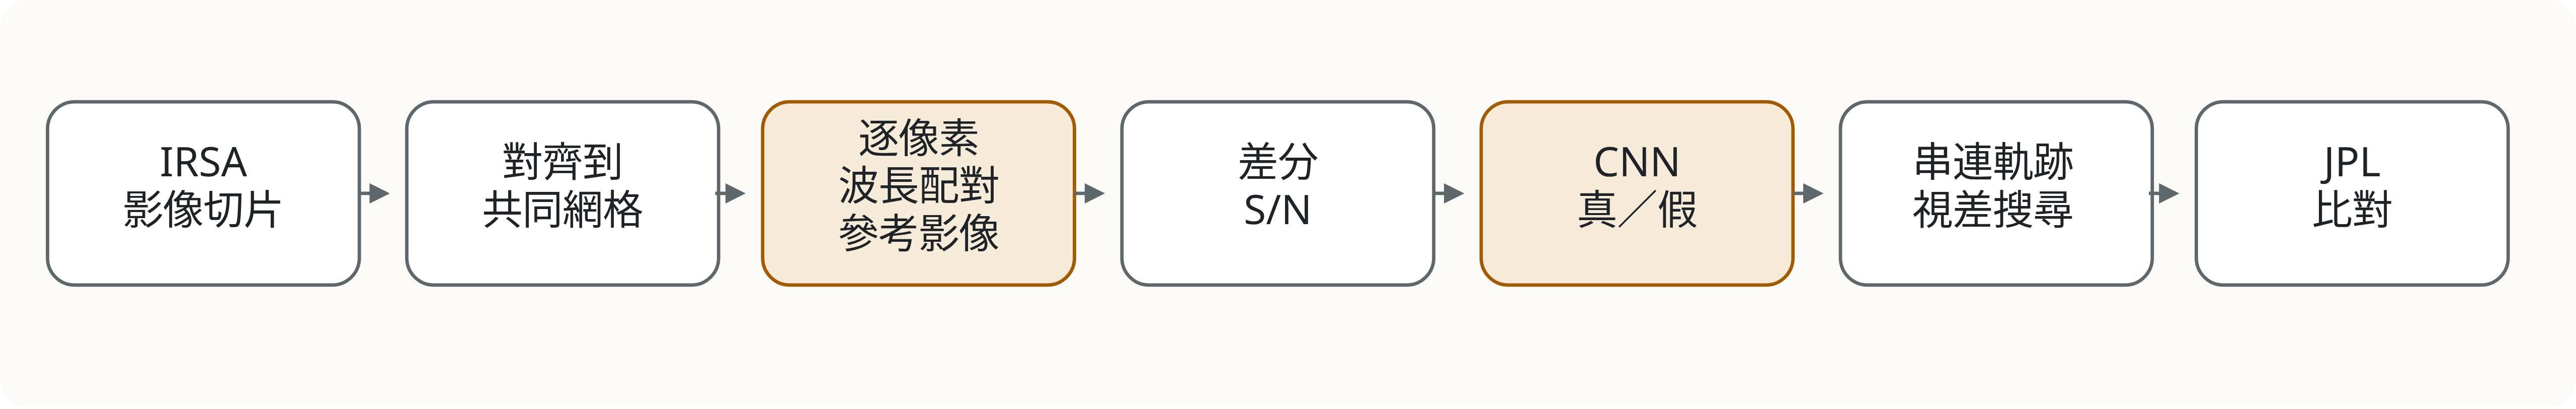
\includegraphics[width=\columnwidth]{svgfig1.png}
\caption{管線。強調的步驟是 SPHEREx 專屬（波長配對的參考影像）或經過學習（CNN）。}
\end{figure}
\subsection{對齊與波長配對的參考影像}
每個 cutout 以雙線性內插重新取樣到 6.15$''$ 像素的切平面網格；覆蓋範圍向內縮 3 像素，帶有硬性壞像素旗標（瞬變、溢位、熱像素、殘影、非線性、溢流、光暈\ldots{}\ldots{}）的像素會被遮罩。對曝光 \emph{i}，每個像素的參考值是同一偵測器、|t\textsubscript{j} $-$ t\textsubscript{i}| $\ge$ 3 小時、且\emph{在該像素} |$\lambda$\textsubscript{j} $-$ $\lambda$\textsubscript{i}| $\le$ 0.03 $\lambda$\textsubscript{i} 的曝光 \emph{j} 的中位數。在 0.5$^\circ$ 的範圍內，濾鏡波長本身就變化約 7\%，所以整張影像用單一波長會混到不同顏色。容差 2\% 時，測試天區有 95\% 的曝光至少有兩張參考影像。

\subsection{差分影像與雜訊模型}
$\alpha$ 是參考影像 S/N 大於 30 的像素上 I/R 的中位數（範圍 0.83--1.13）；n $\ge$ 3 張參考影像時 $\sigma$\textsubscript{R}\textsuperscript{2} = ($\pi$/2) mean($\sigma$\textsubscript{j}\textsuperscript{2})/n；$\varepsilon$ = 0.1。最後一項吸收欠取樣 PSF 造成的恆星殘差。它只能用參考影像的亮度：第一版用了 max(I, R)，結果所有明亮的真實移動天體都被壓在 S/N $\approx$ 1/$\varepsilon$ = 10（第 5.1 節）。S/N $\ge$ 5 的局部極大值成為候選。

\subsection{注入}
模擬天體在重新取樣之前加到原始影像上，使用最近偵測器區域的 PSF，依次像素偏移平移後，從 10 倍過取樣網格合併回像素。每個天區注入 60 個直線移動天體（AB 14--21.5 均勻分布、1--150$''$/小時對數均勻、方向隨機、最多持續 4 天）和 3 個遠距天體（150--800 AU，固定在重心座標系中；它們的視運動來自地球視差）。注入的流量沒有加上自身的光子雜訊。

\subsection{真假訊號網路}
每個候選做成 4 $\times$ 21 $\times$ 21 的小圖：以雜訊為單位的影像、參考影像與 S/N（用 asinh(x/3) 壓縮），加上星表源與鬼影旗標的遮罩。我們刻意不放處理管線的 \texttt{MP\_OUTLIER} 旗標：它會標在真實移動天體上，卻從不出現在注入天體上，網路可能把它學成只在模擬資料成立的捷徑。網路有三個卷積區塊（32/64/128 通道）、平均與最大池化和一個小型 MLP（321,505 個參數），以類別加權的二元交叉熵、AdamW、one-cycle 學習率、90$^\circ$ 旋轉與翻轉訓練 30 個 epoch。資料依天區切分：12 個訓練、2 個驗證（\texttt{ecl120+00}、\texttt{ecl315-12}）、2 個測試（\texttt{ecl180+00}、\texttt{ecl060+00}）。機率在驗證集上做溫度校準（T = 0.780），操作門檻固定在驗證集 1\% 誤報率。

\subsection{串連}
\emph{先找遠距天體。}在每一輪巡天內，把彼此相距 8$''$ 以內、跨越至少 2 個時間點的 $\ge$ 3 個高信心偵測（p $\ge$ 0.5）組成群組。遠距天體在巡天輪次之間的移動，除了地球公轉的視差，還有\emph{它自己的軌道運動}；在數百 AU 處兩者同一個數量級（420 AU 約 150$''$/年）。對每個試驗距離 d（30--3000 AU、1500 個對數間隔值），先預測其他群組在純視差下的位置，接受落在束縛軌道（速度 $\le$ $\surd$2 倍圓軌道速度）可達範圍內的群組，再擬合一個線性漂移，保留讓每個群組都落在 8$''$ 以內的組合。至少需要三輪巡天：只有兩輪時，任何偏移都能被某個漂移吸收，距離與運動無法分開。其中至少一對要相距 $\ge$ 3 像素，否則就是靜止的殘差。之後把落在擬合路徑上的偵測併入，再重新擬合（d、$\mu$\textsubscript{$\alpha$*}、$\mu$\textsubscript{$\delta$}）。\emph{星表輔助。}網站顯示時，比對到 JPL 天體的偵測不論 AI 分數都會參與串連；每條軌跡同時標示「只看 AI 分數的盲連結是否也會找到它」，第 4.5 節報告盲連結的數字。\emph{再找快速移動天體。}剩下的偵測在每輪巡天內串成直線：相隔 0.5 小時到 3 天、速度 0.5--300$''$/小時的配對，至少 4 次偵測、跨越至少 3 個不同的 30 分鐘時段，殘差 $\le$ 8$''$，總位移 $\ge$ 16$''$。這些門檻是在 65 Cybele 天區上設定的；較寬鬆的設定會產生數十個偶然排成一直線的假軌跡。

\section{結果}
\label{sec:results}
\subsection{真實已知小行星（H1）}
\begin{figure}[t]
\centering
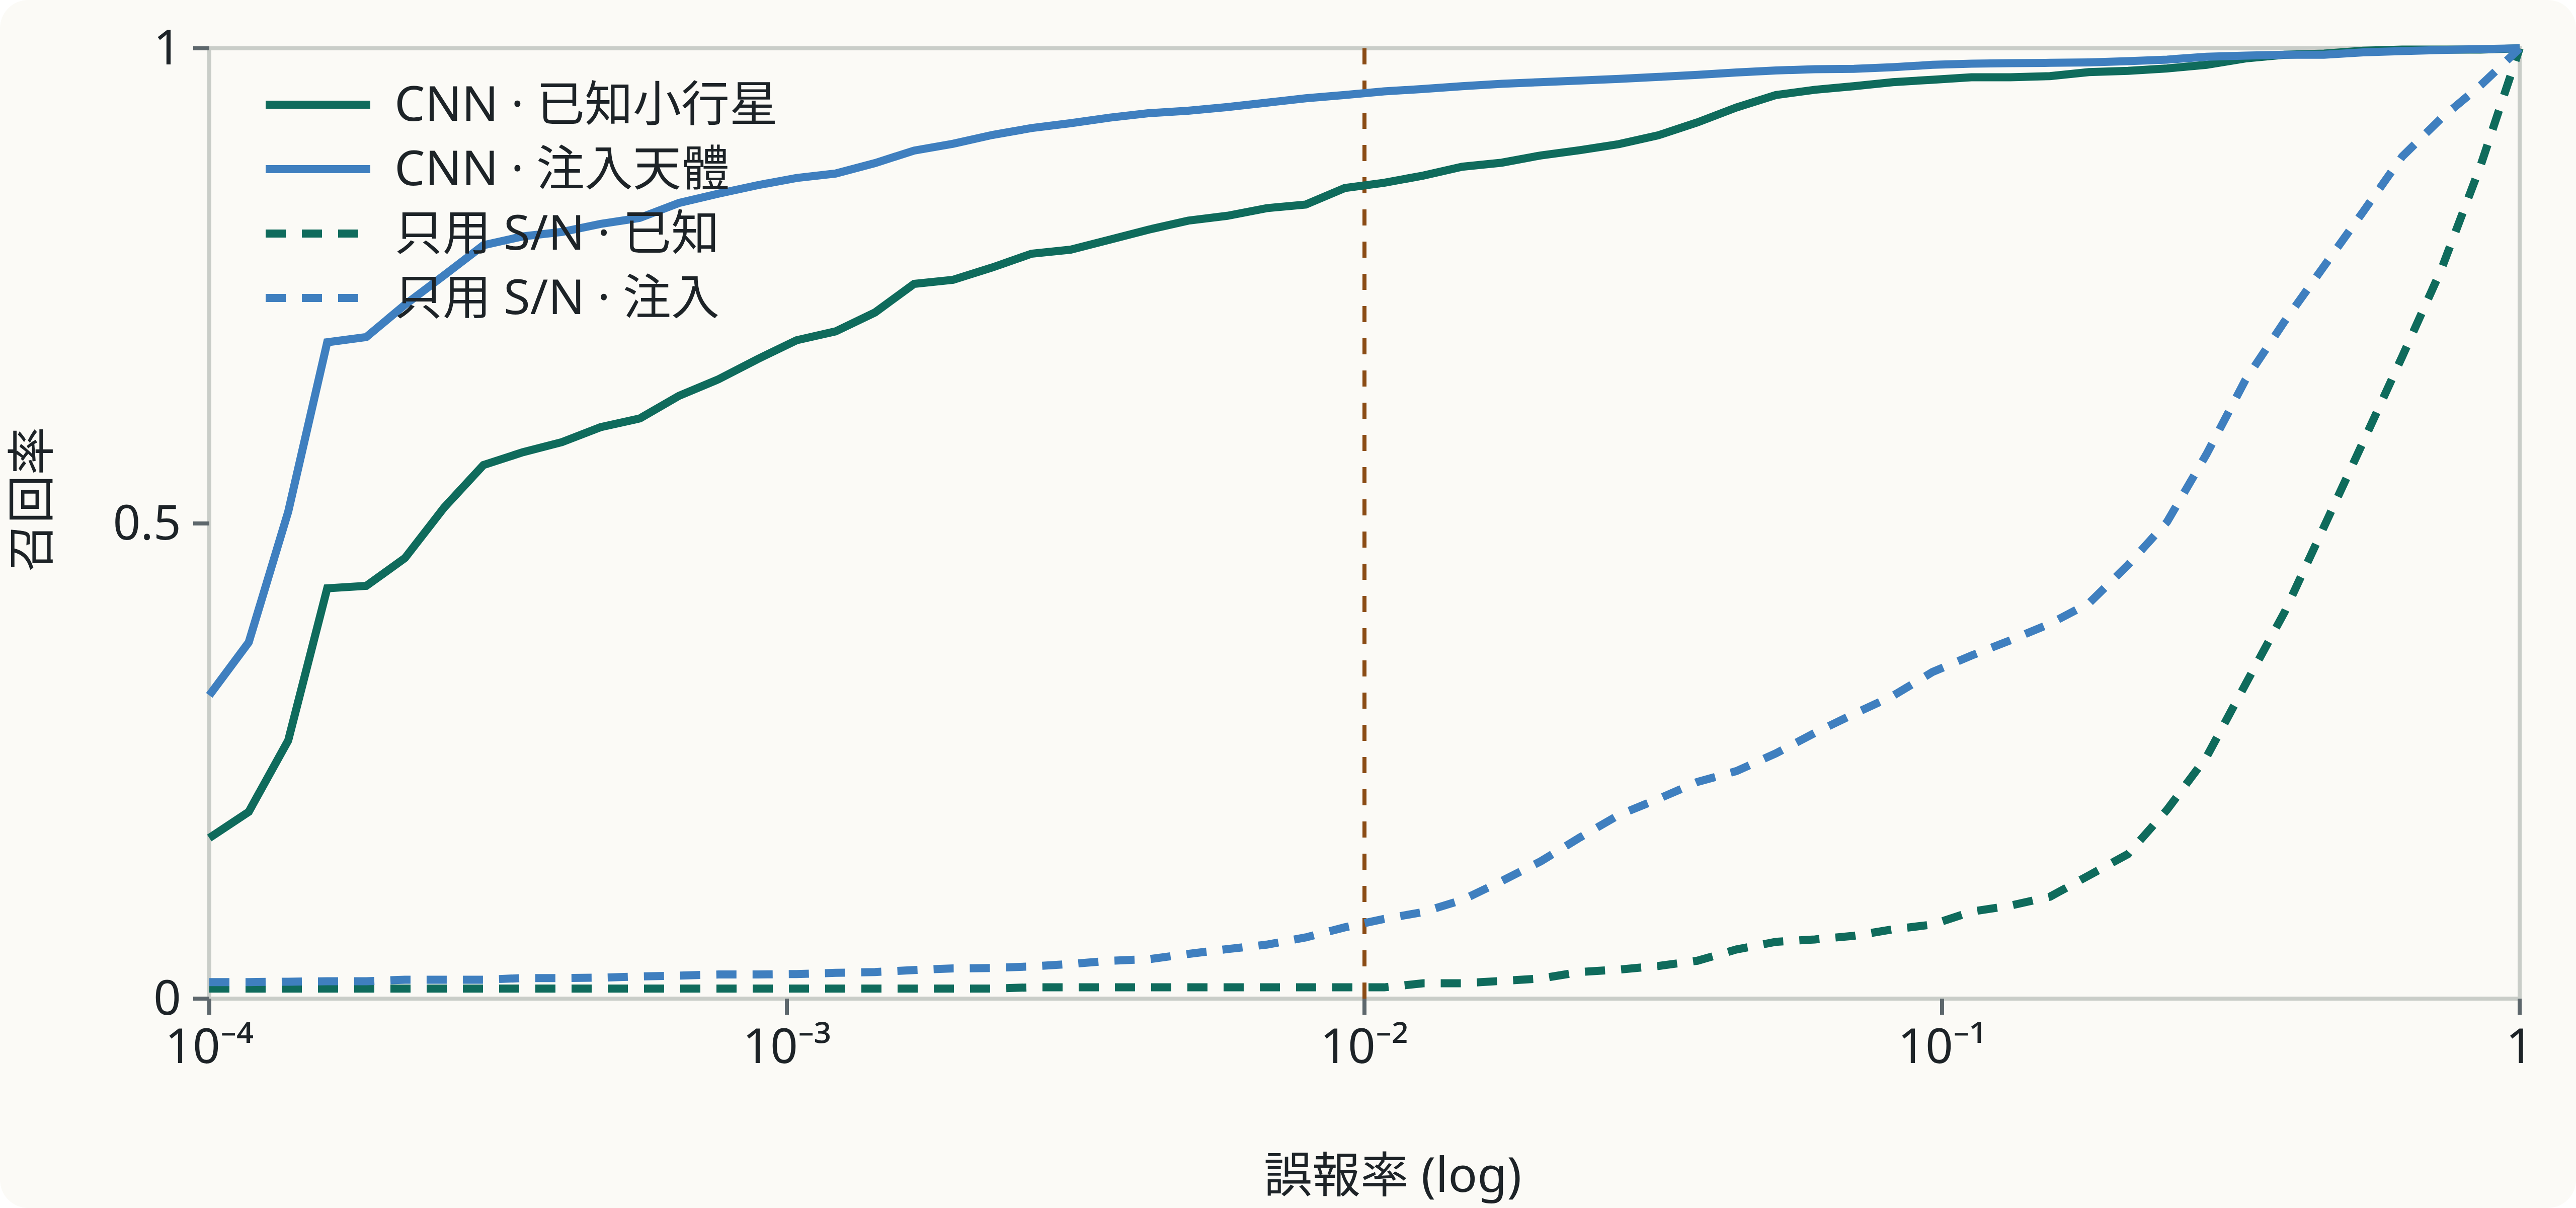
\includegraphics[width=\columnwidth]{svgfig2.png}
\caption{ROC 曲線。實線：CNN；虛線：只看差分影像的 S/N。綠色：755 次真實已知小行星（V $\le$ 18.5）的偵測，對上保留測試天區的假訊號；藍色：測試天區的注入天體。點線：誤報率 1\%。}
\end{figure}
CNN 在真實已知小行星（這些小行星本身從未進入訓練集）上達到 AUROC 0.985（95\% CI 0.981--0.990），在驗證集門檻下召回率 85.3\%（82.6--87.6\%）。只看差分影像的 S/N 等於隨機猜測（AUROC 0.512）：很多假訊號（多半是恆星殘差）和真實移動天體一樣亮。在保留天區的注入天體上，AUROC 為 0.992（0.989--0.994），在誤報率 0.94\% 時召回率 95.1\%。信賴區間以候選為單位重抽樣，沒有涵蓋天區之間的變異。

\emph{更乾淨的比較。}上面的數字合併了 31 個天區的已知小行星，其中 199 次偵測位在訓練天區的影像裡（小行星本身已從訓練集移除），而假訊號只來自兩個測試天區。若只用 CNN 從未訓練過的 19 個驗證、測試與基準天區，並從同一批天區取假訊號（380,000 個），AUROC 為 0.987（0.981--0.992），誤報率 1.15\% 時召回率 90.8\%，只看 S/N 為 0.537。我們以這組數字作為主要結果。

\begin{table}[t]
\centering
\footnotesize

\begin{tabular}{llll}
\hline\hline
V 星等 & n & 召回率 & 95\% CI \\
\hline
< 15 & 111 & 94.6\% & 88.7--97.5\% \\
15--16 & 136 & 99.3\% & 96.0--99.9\% \\
16--17 & 197 & 87.3\% & 81.9--91.2\% \\
17--18.5 & 305 & 75.4\% & 70.3--79.9\% \\
\hline
\end{tabular}
\end{table}
\subsection{各偵測器的誤報（H2）}
\begin{table*}[t]
\centering
\footnotesize

\begin{tabular}{lllllll}
\hline\hline
偵測器 & 波長 & 已知小行星 n & 召回率（95\% CI） & 注入天體召回率 & 假訊號 n & 誤報率 \\
\hline
D1 & 0.75--1.11 $\mu$m & 176 & 79.5\% (73.0--84.8) & 92.6\% & 20,089 & 0.25\% \\
D2 & 1.10--1.64 $\mu$m & 231 & 87.9\% (83.0--91.5) & 95.7\% & 12,960 & 0.24\% \\
D3 & 1.63--2.42 $\mu$m & 122 & 85.2\% (77.9--90.5) & 95.5\% & 10,619 & 0.66\% \\
D4 & 2.40--3.82 $\mu$m & 108 & 86.1\% (78.3--91.4) & 96.1\% & 12,149 & 2.50\% \\
D5 & 3.81--4.42 $\mu$m & 70 & 87.1\% (77.3--93.1) & 93.9\% & 9,268 & 1.06\% \\
D6 & 4.41--5.00 $\mu$m & 48 & 89.6\% (77.8--95.5) & 97.2\% & 7,826 & 1.66\% \\
\hline
\end{tabular}
\end{table*}
整體誤報率符合 1\% 的目標，但並不均勻：長波長的偵測器產生較多高信心的誤報。因此照字面敘述的 H2（每個偵測器都 $\le$ 1.5\%）沒有達成。改用各偵測器各自的門檻可以修正操作點，但我們還沒弄清楚這些偵測器為什麼不同。

\subsection{注入回收完整度}
\begin{figure}[t]
\centering
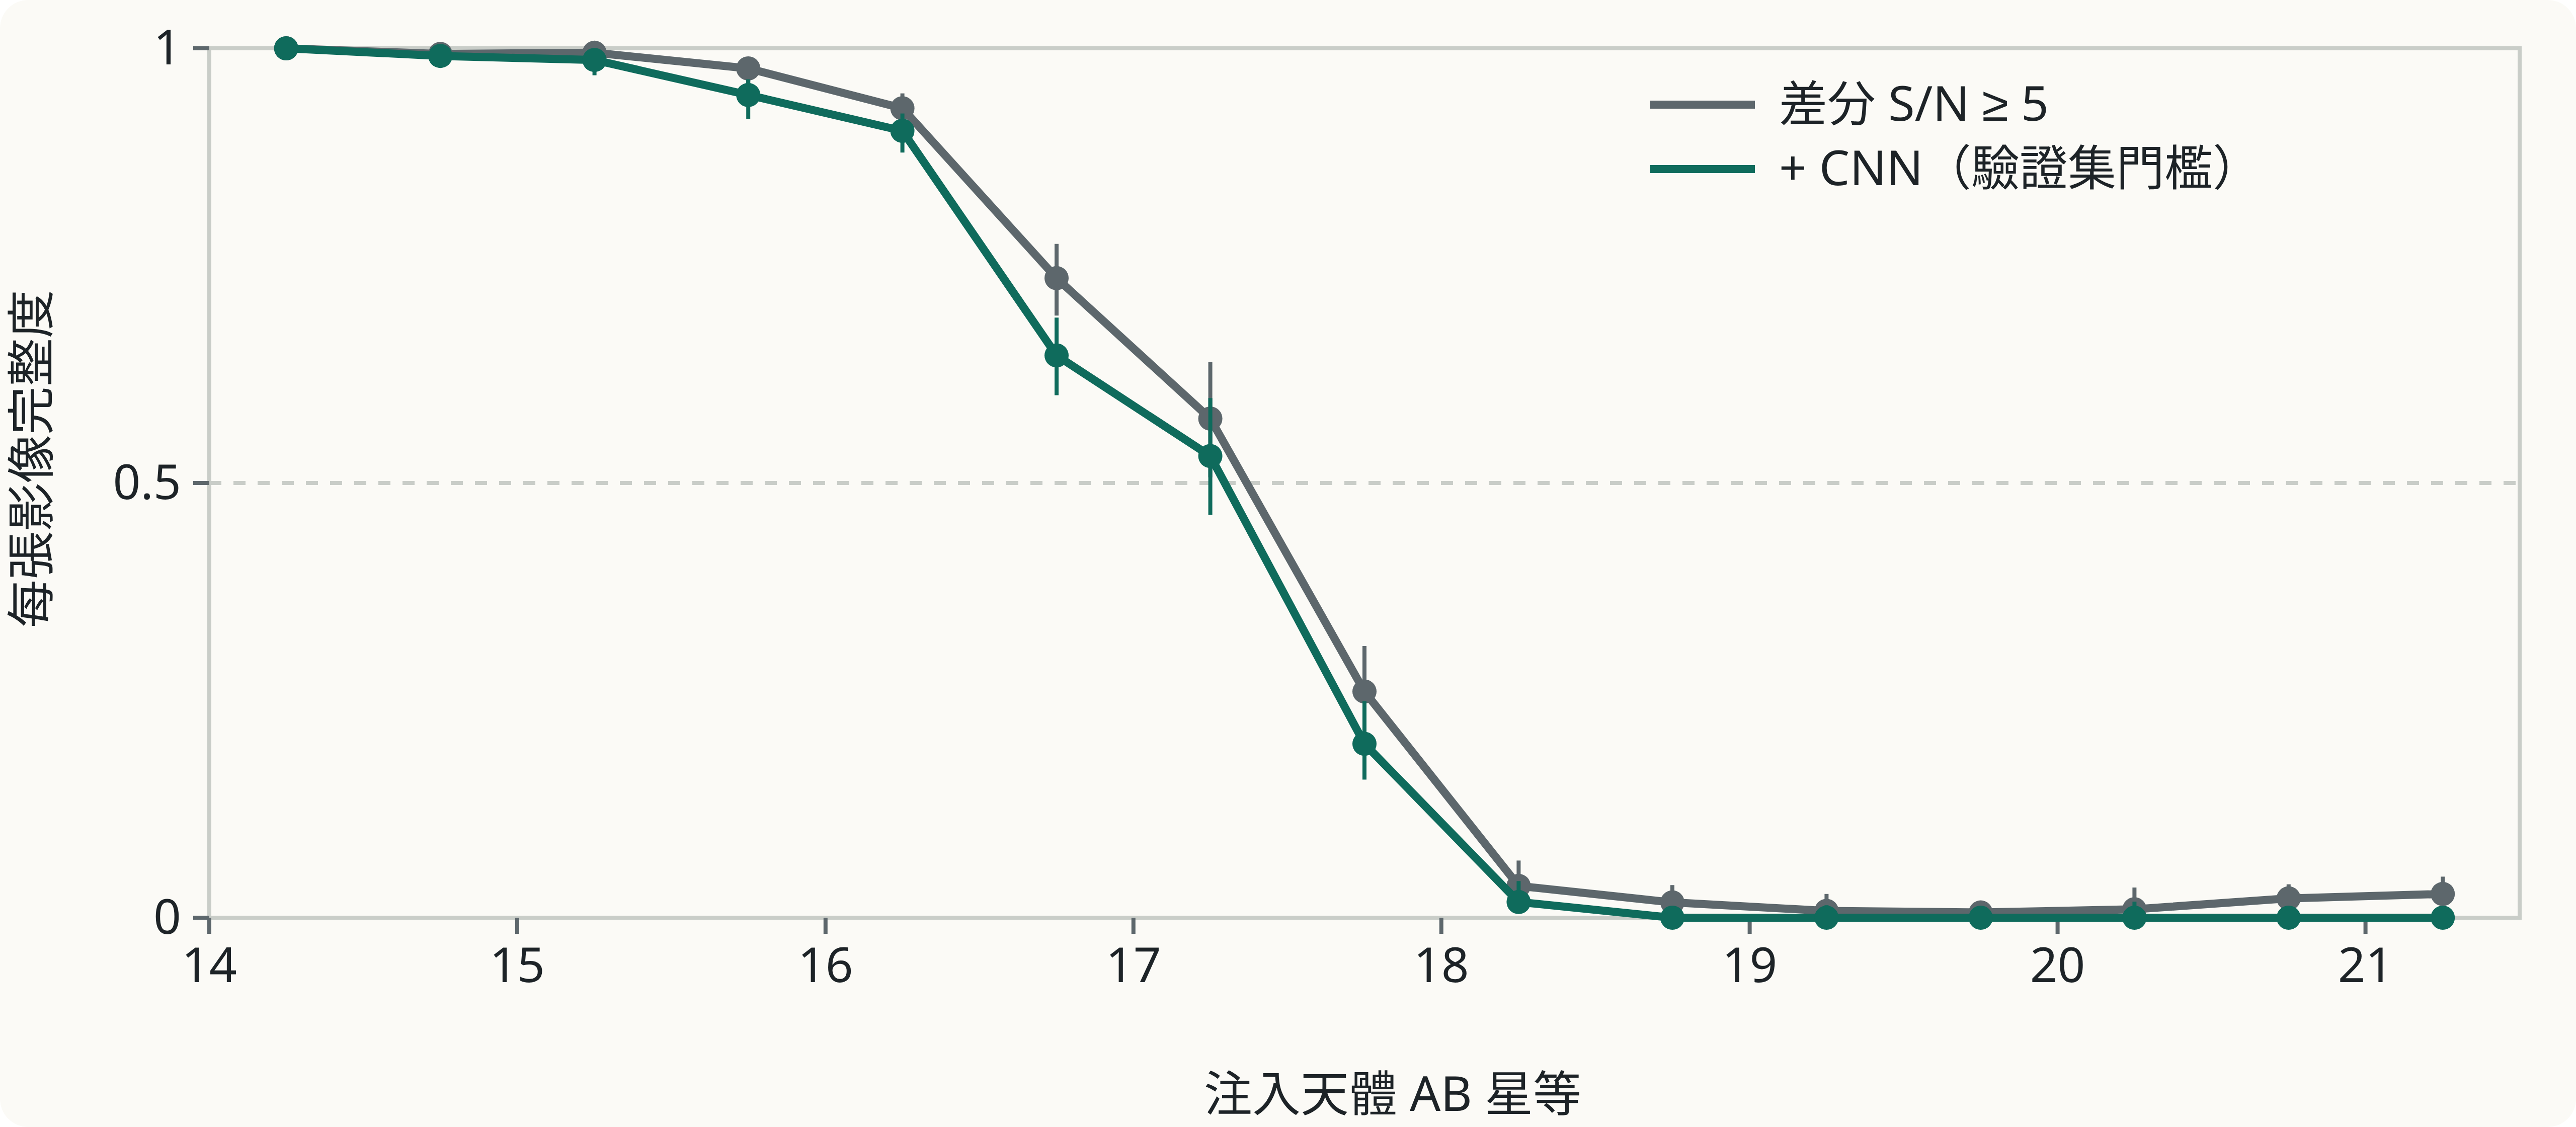
\includegraphics[width=\columnwidth]{svgfig3.png}
\caption{兩個測試天區中注入天體的單張曝光完整度（Wilson 95\% 區間）。CNN 幾乎沒有刪掉真實天體：兩條曲線幾乎重疊。}
\end{figure}
單張曝光中有一半的注入天體在 AB 17.3 被找回。這是單張曝光的極限；比這更暗、但出現在多張曝光中的天體，要靠移位疊加（第 4.7 節）。

\subsection{從視差找到遠距天體（H3）}
\begin{table*}[t]
\centering
\footnotesize

\begin{tabular}{lllll}
\hline\hline
距離 (AU) & AB 15：找回 & AB 16：找回 & AB 17：找回 & 距離誤差中位數 \\
\hline
500 & 4/5 & 4/5 & 4/5 & 0.02\% \\
800 & 4/5 & 4/5 & 3/5 & 0.04\% \\
1500 & 4/5 & 4/5 & 4/5 & 0.09\% \\
3000 & 4/5 & 4/5 & 4/5 & 0.23\% \\
\hline
\end{tabular}
\end{table*}
60 顆注入天體找回 47 顆，距離誤差中位數 0.09\%，最大 37.55\%。搜尋同時也在 5 個天區中的 0 個，產生了 0 條沒有對應任何注入的遠距軌跡；在真正的搜尋中，每一條都需要後續觀測確認。每顆注入天體都沿方向隨機的圓軌道運動，擬合出的軌道運動和注入值相差中位數 0.8$''$/年。依天區來看：在 4 個有三輪巡天的天區找回 47/48 顆；只有兩輪巡天的 1 個天區找回 0/12 顆，這是必然的，因為兩輪時任何偏移都能被某個軌道漂移吸收。另有 1 顆找回的天體距離誤差超過 1\%（最大 38\%）：擬合落在錯誤的距離與運動組合上，第四輪巡天可以打破這種簡併。這個測試的前一版注入的天體沒有軌道運動、擬合也用同一個模型，得到 59/60、距離誤差中位數 0.15\%；那只證明程式和自己的模擬一致。

\subsection{案例}
\textbf{65 Cybele。}在室女座天區，管線把 65 Cybele 的 24 次偵測串成一條速度 24.9$''$/小時的軌跡（JPL 給的是 24$''$/小時）。這個天區顯示 7 條軌跡，但其中 3 條要靠星表輔助才串得起來；只看 AI 分數的盲連結找到 4 條，其中 3 條是已知小行星。逐條和 JPL 比對，4 條一致，2 條混入了不相關的偵測（網站上有標示）。\textbf{模擬行星。}一顆注入在 420.0 AU（AB 15.5）的天體，在真實影像中被找回成一條軌跡：327 次偵測、跨越 4 輪巡天，擬合距離 420.2 AU。

\begin{figure*}[t]
\centering
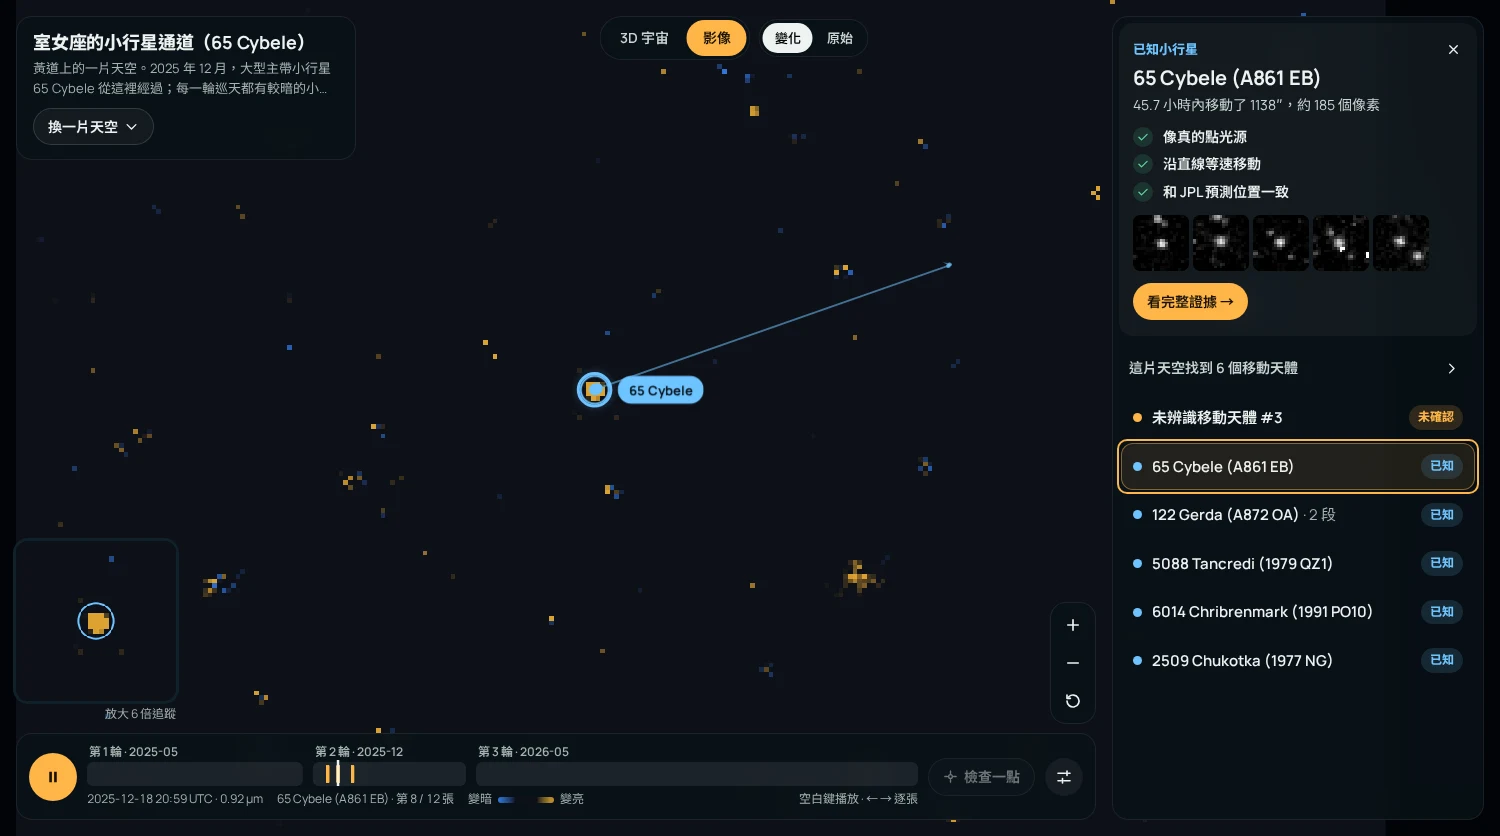
\includegraphics[width=0.95\textwidth]{img_viewer_zh.png}
\caption{公開檢視器：追蹤 65 Cybele 時的差分影像（琥珀色 = 比參考影像亮）。}
\end{figure*}
\subsection{以 SPHEREx 為觀測者，和 JPL 比對天體測量}
對每條以已知天體命名的軌跡，我們向 JPL Horizons 查詢每次偵測時刻、以 SPHEREx 太空船（Horizons ID $-$163182）為觀測者的天體位置；在低地球軌道上，光是觀測者位置就會讓主帶小行星移動最多約 5$''$。在和 JPL 一致的軌跡中，6 個天體的 78 次偵測和預測相差中位數 0.7$''$（一個 6.15$''$ 像素的 0.11；第 90 百分位 1.47$''$）。另有 3 條命名軌跡有四分之一以上的偵測遠離 JPL 位置，標為混入而不計入。

\subsection{真實矮行星的距離}
海王星外的矮行星在半年內被視差帶著移動 1--2$^\circ$，超出一片天區，所以我們依 JPL 星曆在每一輪巡天各開一片 0.6$^\circ$ 天區，跑同一套管線，再把三輪的 AI 候選（分數 $\ge$ P\_LINK，不使用任何星表）合在一起做遠距搜尋。\textbf{鳥神星}：盲搜尋在整片資料裡只連出 1 條遠距軌跡，就是它（56 次偵測、三輪），擬合距離 52.71 AU，JPL 為 52.72 AU（差 0.02\%）。\textbf{妊神星}：同樣只有 1 條，49.49 AU 對 49.82 AU（差 0.66\%）。\textbf{鬩神星}（95.52 AU，V $\approx$ 18.7）在單張影像中完全偵測不到；移位疊加也沒有找回它，因為它在一輪巡天的兩週內，自己的軌道運動就移動約 9 個像素，而我們的疊加只補償視差（為 150 AU 以外、幾乎不動的天體設計）。為了讓鳥神星在近處也連得起來，連結步驟加入了「慢速短軌跡」與曲率容許；這一版在 12 顆遠距天體同時存在的天區會把不同天體混在一起，第 4.4 節的網格因此一度退步到 45 條假軌跡。改成先找「同一位置」的偵測群、剩下的才組短軌跡，並要求連結後所有偵測都落在同一條路徑上，網格回到 0 條假軌跡、距離誤差中位數 0.09\%（表 4 已是修正後的結果）。

\subsection{移位疊加}
對每輪巡天與 36 個試驗距離（40--3000 AU），把差分 S/N 影像沿預測的視差路徑移回該輪中間時刻再相加。第一版直接相加 S/N，注入測試只找回 3/36 顆，並產生約 800 條假軌跡：單張差分影像的雜訊有很重的尾巴（1.3\% 的像素超過 3$\sigma$，來自小行星、宇宙線與相減殘差），疊加後會堆成大量假峰值，連結時還會搶走真天體的峰值。修正後每張影像先截在 $\pm$3$\sigma$（暗天體每張只有約 1$\sigma$，不受影響），疊加圖再除以自己的穩健雜訊，連結容許誤差收緊到 4$''$，並在連出的距離上重新疊加確認每個峰值。在三片不擁擠、未用於訓練的天區注入 AB 18--20.5、500 與 1500 AU 的天體：AB 18--19 找回 14/18，AB $\ge$ 19.5 找回 0/18，50\% 完整度約 AB 19.2，比單張影像深約 2 等；沒有假軌跡（0 條）。

\subsection{沿 Planet Nine 預測路徑的搜尋}
依 Brown \& Batygin（2021）中位數軌道在天球上的路徑，以及 Brown 等（2024）指出尚未被排除的區域，我們在 A 區（RA 75--105$^\circ$，北銀河面交會）、B 區（RA 45--74$^\circ$，遠日點附近）沿路徑每 1.5$^\circ$ 取一片 0.5$^\circ$ 天空，並在 Phan 等（2025）IRAS/AKARI 候選外推到 2025 年的位置附近取 3$\times$3 片（D 區），只保留至少有三輪巡天的天空：A 3、B 20、D 9 片，扣除星點遮罩後共 7.89 平方度。這是沿路徑的取樣，不是覆蓋整條 $\pm$12$^\circ$ 的機率帶。

\emph{單張影像。}32 片天空的遠距搜尋都沒有連出任何軌跡（0 條）。\emph{疊加。}共連出 63 條軌跡，集中在最靠近銀河面、最擁擠的天區。逐條檢查（至少三輪、擬合殘差、束縛軌道、非靜止、距離不在邊緣、JPL 已知天體、三輪亮度一致）後，23 條因亮度不一致、1 條因與已知小行星重合被排除，39 條全部通過。為了估計巧合，我們把各輪的時間標籤循環互換後重新連結與確認------這在物理上不可能對應真實天體------得到 55 與 60 條（平均 57.5），而真實時間是 63 條：差距在 Poisson 起伏之內。因此這些軌跡整體上和擁擠星場中的巧合排列無法區分，我們不把其中任何一條列為候選。

\emph{上限。}在這 7.89 平方度裡，沒有比 AB 約 17 更亮、距離 30--3000 AU 的天體；到 AB 19.2 也沒有能和巧合區分開的天體。疊加的完整度是在不擁擠的天區量得的，銀河面附近的實際完整度較低。若粗略套用 Planet Nine 的預測亮度分布（V = 22.0 +1.1/$-$1.4，Brown 等 2024），只有約 2.3\% 的情況會比 AB 19.2 亮（近紅外顏色未知，甲烷吸收會讓它更暗），所以這次非偵測是預期中的結果，對 Planet Nine 幾乎沒有約束力。

\section{討論}
\label{sec:discussion}
\subsection{縮小模擬與真實之間的落差}
我們第一次在「已知小行星」上的評估只得到 AUROC 0.66。背後有三個獨立的問題，只有一個出在網路本身。（1）\emph{標籤。}大多數被比對到的「已知」天體 V $\approx$ 20，遠比單張曝光能看到的暗；它們的預測位置只是剛好落在恆星殘差上。現在我們只計入在 1.5 像素內相符、V $\le$ 18.5 的天體，並且加入了亮小行星天區。（2）\emph{雜訊模型。}系統誤差項用了 max(I, R)，把明亮的真實移動天體壓在 S/N $\approx$ 10。（3）\emph{捷徑。}第 2 級處理管線會在真實移動天體上設定 \texttt{MP\_OUTLIER}；注入天體從來沒有。把它從輸入中拿掉，網路才必須學會辨認形態。現在網站把這個旗標當成獨立證據顯示。

\subsection{限制}
\begin{itemize}
\item QR3 的注入使用 QR2 的 PSF 立方體；注入的天體沒有加上光子雜訊。
\item 已知天體的位置最多線性外推 0.25 天；暗端的召回率可能被低估。
\item 信賴區間是以候選重抽樣，不是以天區；只有兩個測試天區，天區之間的變異沒有被涵蓋。
\item 串連門檻是在兩個同時作為案例的天區上調整的。
\item 各偵測器的誤報率相差一個數量級（表 3）。
\item 示範用的行星刻意調亮（AB 15.5）。真正的遙遠行星會遠比我們的單張曝光極限暗。
\item 移位疊加只補償視差，不搜尋軌道運動；150 AU 以內的天體（例如鬩神星）在一輪巡天內會被自己的運動拖糊。疊加的完整度是在不擁擠的天區量得的。
\item 第 4.9 節的巧合估計只用兩種時間互換；搜尋天區是沿預測路徑的取樣，不是整條機率帶。
\item 軌道運動在約一年的基線上以線性漂移近似，適用於約 100 AU 以外，不適用於更近的天體。
\item 網站上顯示的軌跡包含星表輔助的連結；第 4.5 節的盲連結數字才是管線本身的表現。
\item 圖 2 的已知小行星 AUROC 把訓練天區影像中的正樣本和兩個測試天區的負樣本混在一起；第 4.1 節的同天區比較較為乾淨。
\end{itemize}

\subsection{要真的找到 Planet Nine 還缺什麼}
單張影像（AB 約 17）與移位疊加（AB 約 19.2）都比 Planet Nine 的預測亮度 V $\approx$ 22 淺 3 等以上。更深需要：把一輪巡天內不同波段疊成寬波段（每個天體約有數百張曝光）、在疊加中同時搜尋軌道運動，以及更多輪巡天（SPHEREx 每半年一輪，第四輪可以打破距離與運動的簡併）。擁擠星場是另一個瓶頸：第 4.9 節的巧合率顯示，銀河面附近需要更好的恆星相減，才能讓真正的訊號從巧合中凸顯出來。任何候選都必須由更大的望遠鏡後續觀測確認，並依 MPC 的規定（SPHEREx 的觀測站代碼為 288）回報。

\section{結論}
\label{sec:conclusions}
波長配對的差分讓 SPHEREx 可以用於變化偵測。只用模擬資料訓練的網路，在修正標籤、雜訊模型與處理管線旗標捷徑之後，可以轉移到真實小行星上。在至少三輪巡天的天區，同時擬合視差與軌道運動，能找回沿真實軌道運動的注入遠距天體，也能只靠 SPHEREx 的視差把真實矮行星的距離量到 1\% 以內。沿 Planet Nine 預測路徑的搜尋沒有找到能和巧合區分的天體，並給出這片天空的亮度上限。公開工具讓大眾看到的，是經過這些量測步驟之後的結果，而不是未經處理的閃爍影像。

\section*{開放研究}
程式碼（管線、訓練、評估與網站）在專案儲存庫的 \texttt{spherex/} 底下。SPHEREx 影像可在 NASA/IPAC IRSA 公開取得；已知天體資料來自 JPL SSD API。本文每個數字都由 \texttt{scripts/build\_paper\_evidence.py} 與 \texttt{scripts/render\_paper.py} 從下列檔案產生。雜湊值只能證明這些檔案在渲染之後沒有被修改，不能證明它們建立的時間。公開發布的網路（\texttt{/models/rb\_cnn.pt}）與其評估指標可以下載；訓練檢查點與原始分數檔不對外提供。

\begin{table}[t]
\centering
\footnotesize

\begin{tabularx}{\columnwidth}{Xl}
\hline\hline
檔案 & SHA-256（前 12 碼） \\
\hline
\texttt{paper\_evidence/evidence.json} & \texttt{e145327c9a66} \\
\texttt{models/metrics.json} & \texttt{3fba3faee765} \\
\texttt{models/recovery.json} & \texttt{f802fbe4a5c4} \\
\texttt{models/rb\_cnn.pt} & \texttt{eca4e82ba7de} \\
\texttt{paper\_evidence/planetx\_grid.json} & \texttt{0d9835794331} \\
\hline
\end{tabularx}
\end{table}
證據檔案：evidence.json $\cdot$ planetx\_grid.json $\cdot$ metrics.json $\cdot$ recovery.json。

\textbf{資料致謝。}本研究使用 NASA SPHEREx 任務的資料，經由 NASA/IPAC 紅外線科學資料庫取得，以及 JPL Small-Body Identification API。本作品是黑客松原型，未經 NASA 背書。

\section*{附錄}
\subsection*{A. 假說、判準與偏離}
\begin{table*}[t]
\centering
\footnotesize

\begin{tabularx}{\textwidth}{lXXXl}
\hline\hline
假說 & 判準 & 設定時點 & 結果 & 是否達成 \\
\hline
H1 & 真實已知小行星 AUROC $\ge$ 0.95，且誤報率 1\% 時召回率 $\ge$ 80\% & 2026-10-20，訓練前（PLAN.md G3） & AUROC 0.985 (0.981--0.990); recall 85.3\% (82.6--87.6\%) & 達成 \\
H2 & 每個偵測器的誤報率 $\le$ 1.5\%（驗證集門檻） & 2026-10-21，看過整體誤報率之後（事後設定） & 0.94\% overall; D2 0.24\% -- D4 2.50\% & 未達成 \\
H3 & 注入遠距天體的距離誤差 $\le$ 2\% & 2026-10-21，注入網格執行前（WEB\_PAPER\_PLAN.md） & 47/60 recovered; median 0.09\%, max 37.55\% & 部分達成 \\
\hline
\end{tabularx}
\end{table*}
\textbf{與原計畫的偏離。}（a）為了節省運算，亮小行星基準集在 20 個天區中做到第 15 個就停止。（b）檢查早期結果後，已知天體標籤的星等上限從 V $\le$ 21.5 改為 V $\le$ 18.5。（c）在那次結果之後拿掉了 outlier 旗標通道並修正雜訊模型，網路從頭重新訓練。（d）軌跡串連的門檻是在示範天區上設定的。

\subsection*{B. 設定}
天區大小 0.5$^\circ$（使用者提交的天區為 0.3$^\circ$）；cutout 為天區的 1.5 倍；參考影像：最多 36 張候選曝光、波長容差 3\%、相隔 $\ge$ 3 小時；$\varepsilon$ = 0.1；偵測 S/N $\ge$ 5、5 $\times$ 5 局部極大值；小圖 21 像素；訓練 30 個 epoch、批次 512、學習率 10\textsuperscript{$-$3}、正樣本權重 $\le$ 20；串連容差 8$''$、p $\ge$ 0.5。

\section*{致謝}
本文使用 SPHEREx 的資料產品。SPHEREx 是美國噴射推進實驗室與加州理工學院的聯合計畫，由 NASA 資助。資料取自 NASA/IPAC 紅外線科學檔案館（IRSA）：DR1（doi:10.26131/IRSA678）、QR3（doi:10.26131/IRSA662）、QR2（doi:10.26131/IRSA652）。本文亦使用歐洲太空總署 Gaia 任務的資料，由 Gaia DPAC 處理。

\section*{參考文獻}
\begin{list}{}{\leftmargin=1.5em\itemindent=-1.5em\itemsep=2pt\small}
\item Astropy Collaboration et al. (2022). The Astropy Project: sustaining and growing a community-oriented open-source project. \emph{ApJ}, 935, 167.
\item Batygin, K., \& Brown, M. E. (2016). Evidence for a distant giant planet in the Solar System. \emph{AJ}, 151, 22.
\item Brown, M. E., \& Batygin, K. (2021). The orbit of Planet Nine. \emph{AJ}, 162, 219.
\item Brown, M. E., Holman, M. J., \& Batygin, K. (2024). A Pan-STARRS1 search for Planet Nine. \emph{AJ}, 167, 146.
\item Phan, T. L., Goto, T., et al. (2025). A search for Planet Nine with IRAS and AKARI data. \emph{PASA}; arXiv:2504.17288.
\item Minor Planet Center. Reporting observations (ADES) and observatory codes. https://docs.minorplanetcenter.net/
\item Doré, O., et al. (2014). Cosmology with the SPHEREX all-sky spectral survey. arXiv:1412.4872.
\item Duev, D. A., et al. (2019). Real-bogus classification for the Zwicky Transient Facility using deep learning. \emph{MNRAS}, 489, 3582.
\item Guo, C., Pleiss, G., Sun, Y., \& Weinberger, K. Q. (2017). On calibration of modern neural networks. \emph{ICML}.
\item Kuchner, M. J., et al. (2017). The first brown dwarf discovered by the Backyard Worlds: Planet 9 citizen science project. \emph{ApJL}, 841, L19.
\item NASA/IPAC Infrared Science Archive. SPHEREx Quick Release data and image-cutout service documentation.
\item JPL Solar System Dynamics. Small-Body Identification API (sb\_ident).
\end{list}

\end{document}
